\documentclass[10pt,a4paper,landscape]{article}
\usepackage[margin=10mm]{geometry}
\usepackage[T1]{fontenc}
\usepackage{lmodern}
\usepackage{array,booktabs,tabularx,ragged2e,amsmath}
\usepackage{tikz}
\usetikzlibrary{arrows.meta}
\usepackage[colorlinks=true,urlcolor=blue,linkcolor=blue]{hyperref}
\pagestyle{empty}
\setlength{\parindent}{0pt}
\setlength{\tabcolsep}{4pt}
\setlength{\intextsep}{3pt}
\setlength{\textfloatsep}{3pt}
\newcolumntype{Y}{>{\RaggedRight\arraybackslash}X}

\begin{document}
{\large\bfseries CubeSat image dataset: camera and independent pose reference alternatives}\par
\smallskip
{\small Assumptions: two cooperative spacecraft in low Earth orbit, with a star tracker and an IMU on each. Reference pose uses GNSS and attitude telemetry. No visual targets or docking features are added. Linked option names lead to sources.}

\begin{table}[!ht]
\centering
\small
\renewcommand{\arraystretch}{1.08}
\begin{tabularx}{\linewidth}{@{}>{\RaggedRight\arraybackslash}p{44mm}YY@{}}
\toprule
\textbf{Alternative} & \textbf{Capability or measurement method} & \textbf{Mission implication} \\
\midrule
\multicolumn{3}{@{}l}{\textbf{Image cameras (each meets the $1920\times1200$ minimum)}} \\
\addlinespace[2pt]
\href{https://projects.au.dk/ausat/delphini1/images}{\textbf{C1. GomSpace NanoCam C1U}}
& $2048\times1536$ RGB CMOS. Demonstrated in orbit on Delphini-1.
& Heritage reference. The \href{https://gomspace.com/product/nanocam-c1u/}{manufacturer lists it as phased out}. Verify exposure timing and shutter mode, and focus the optics for proximity. \\
\addlinespace[3pt]
\href{https://www.msss.com/files/ECAM-C50_M50.pdf}{\textbf{C2. MSSS ECAM-C50}}
& $2592\times1944$ RGB, rolling shutter. Native format: 2.8 frames/s over 200 Mbit/s SpaceWire. Imaging power: 1.6 W.
& Flight proven on OSIRIS-REx. Rolling shutter needs motion assessment. Optics and baffle can dominate the CubeSat volume allocation. \\
\addlinespace[3pt]
\href{https://softwareservices.flir.com/BFS-U3-51S5/latest/Model/spec.html}{\textbf{C3. FLIR Blackfly S}\newline BFS-U3-51S5C-C}
& $2448\times2048$ RGB, global shutter. Up to 73 frames/s in 8-bit Bayer format. 36 g without lens, 3 W maximum.
& Compact industrial camera with hardware I/O for synchronization. Requires mission qualification for radiation, vacuum and temperature. \\
\midrule
\multicolumn{3}{@{}l}{\textbf{Independent reference sensors and algorithms (exclude the training images from label generation)}} \\
\addlinespace[2pt]
\href{https://navi.ion.org/content/71/3/navi.661}{\textbf{G1. Raw carrier-phase GNSS on both spacecraft}}
& Relative translation and range. Double-differenced carrier phase $\rightarrow$ LAMBDA integer ambiguity resolution $\rightarrow$ weighted position solution and optional offline smoothing.
& Pair with G2 for full pose. Requires common GNSS visibility and validated ambiguity fixes. A published CubeSat hardware ground test achieved about 1.5 cm position RMSE. This is not an orbital accuracy guarantee. \\
\addlinespace[3pt]
\href{https://www.aac-clyde.space/wp-content/uploads/2021/11/ST200-1.pdf}{\textbf{G2. Existing star trackers and IMUs}}
& Body attitude in a common inertial frame. Star tracker quaternions and IMU gyro rates $\rightarrow$ multiplicative extended Kalman filter (MEKF) or offline attitude smoother $\rightarrow$ relative rotation composition.
& Uses existing sensors. Estimate gyro bias and calibrate sensor and camera alignments. Relative pose uncertainty includes both attitude solutions, synchronization error and mounting drift. Validate tracker coverage over the required slew rates. \\
\bottomrule
\end{tabularx}
\end{table}

\smallskip
\textbf{Pose label generation with G1 + G2}\par
\smallskip
\begingroup
\centering
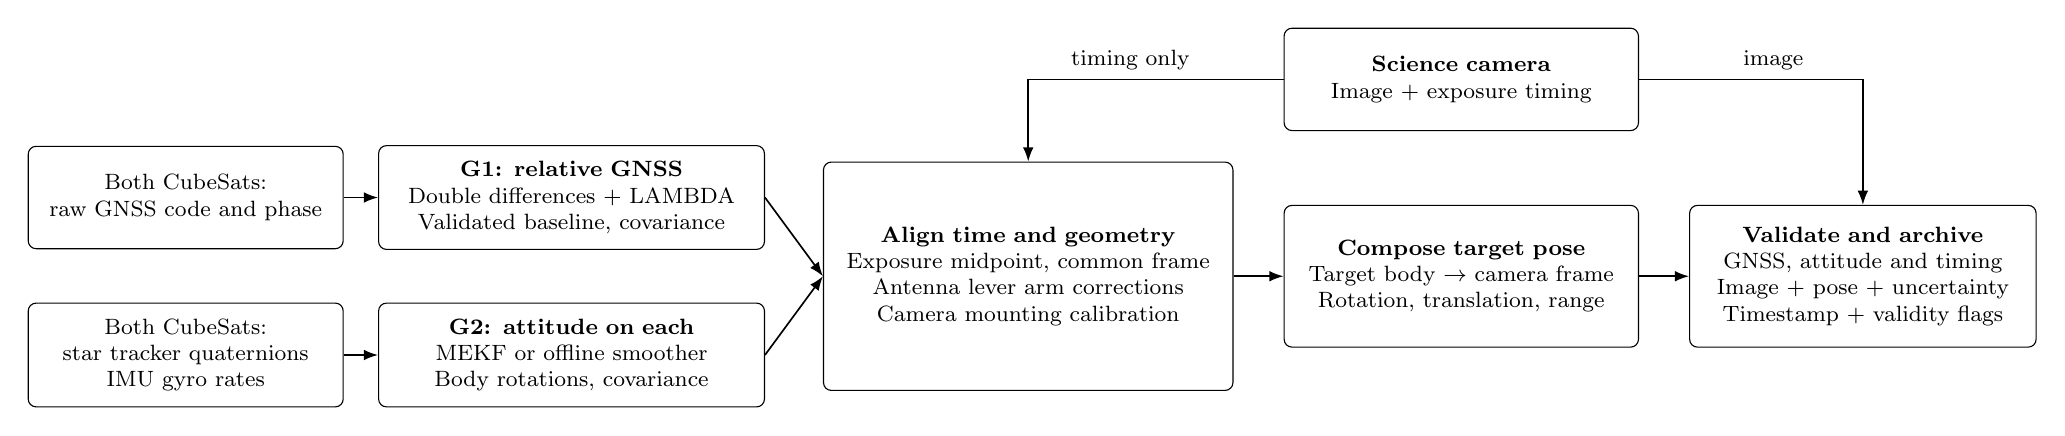
\begin{tikzpicture}[
  x=1mm,y=1mm,font=\footnotesize,
  block/.style={draw,rounded corners=1mm,align=center,inner sep=2mm,
    text width=36mm,minimum height=13mm},
  arrow/.style={-{Latex[length=1.8mm]},semithick}
]
\node[block] (gnss) at (0,0) {Both CubeSats:\\raw GNSS code and phase};
\node[block] (attitude) at (0,-20) {Both CubeSats:\\star tracker quaternions\\IMU gyro rates};
\node[block,text width=45mm] (g1) at (49,0) {\textbf{G1: relative GNSS}\\Double differences + LAMBDA\\Validated baseline, covariance};
\node[block,text width=45mm] (g2) at (49,-20) {\textbf{G2: attitude on each}\\MEKF or offline smoother\\Body rotations, covariance};
\node[block,text width=48mm,minimum height=29mm] (align) at (107,-10) {\textbf{Align time and geometry}\\Exposure midpoint, common frame\\Antenna lever arm corrections\\Camera mounting calibration};
\node[block,text width=41mm,minimum height=18mm] (pose) at (162,-10) {\textbf{Compose target pose}\\Target body $\rightarrow$ camera frame\\Rotation, translation, range};
\node[block,text width=40mm,minimum height=18mm] (labels) at (213,-10) {\textbf{Validate and archive}\\GNSS, attitude and timing\\Image + pose + uncertainty\\Timestamp + validity flags};
\node[block,text width=41mm] (camera) at (162,15) {\textbf{Science camera}\\Image + exposure timing};
\draw[arrow] (gnss) -- (g1);
\draw[arrow] (attitude) -- (g2);
\draw[arrow] (g1.east) -- (align.west);
\draw[arrow] (g2.east) -- (align.west);
\draw[arrow] (align) -- (pose);
\draw[arrow] (pose) -- (labels);
\draw[arrow] (camera.west) -| node[pos=0.3,above] {timing only} (align.north);
\draw[arrow] (camera.east) -| node[pos=0.3,above] {image} (labels.north);
\end{tikzpicture}\par
\endgroup
\smallskip
\begin{minipage}{\linewidth}
\footnotesize
\textbf{Frame composition.} Let $O$ denote the observer body, $T$ the target body, $C$ the camera and $I$ a common inertial frame. The transform ${}^{X}\!T_Y$ maps points from $Y$ to $X$. G1 supplies the differential translation, G2 supplies the body rotations, and calibrated antenna offsets locate the body origins. Use the calibrated camera transform ${}^{O}\!T_C$ for the active optical setting.
\[
{}^{C}\!T_T = \left({}^{I}\!T_O\,{}^{O}\!T_C\right)^{-1}{}^{I}\!T_T,
\qquad
\text{distance} = \left\|{}^{C}\!\mathbf t_T\right\|.
\]
\textbf{Operation and validation.} Process synchronized telemetry offline, or exchange it over an intersatellite link for onboard processing. Image pixels enter only the archive. Calibrate camera intrinsics and sensor geometry. Publish timestamps, covariance and validity flags.\par
\smallskip
\textbf{Literature reference.} \href{https://doi.org/10.1109/AERO53065.2022.9843439}{SPEED+ (Sec.~5, p.~8, Eq.~4)} uses calibration-based scoring thresholds of $\theta_t=2.173\,\mathrm{mm/m}$ for normalized three-dimensional translation and $\theta_q=0.169^\circ$ for rotation. Adopt these as provisional total label error ceilings: $B_t(r)=2.173\times10^{-3}r$ and $B_q=0.169^\circ$, where $r$ is camera-to-target range. Lateral error shares the total translation budget. These thresholds specify neither a confidence level nor a one-pixel criterion.\par
\smallskip
\textbf{Close range implication.} \href{https://doi.org/10.1007/978-3-031-25056-9_8}{CubeSat-CDT (Table~2, p.~116)} reports real-image ranges of 0.65--1.2~m, yielding $B_t=1.41$--$2.61$~mm under the adopted criterion. Its Table~4 (p.~122) reports model prediction errors. The paper does not quantify label uncertainty. The cited 15~mm GNSS RMSE does not demonstrate this accuracy. Allocate and validate contributions from GNSS, attitude, timing and calibration with stated confidence and margin.
\end{minipage}

\clearpage
{\large\bfseries Complement: optical field of view and 2U framing distance}\par
\smallskip
\small
\textbf{Geometry (nominal pinhole model).} Use the bare \href{https://www.cubesat.org/s/CDS-REV14_1-2022-02-09.pdf}{CDS Rev.~14.1, Appendix~B, 2U drawing} envelope, $W\times D\times L=0.100\times0.100\times0.227$~m, including the rail ends. The target body center lies on the camera boresight. Distances below are from the camera optical center to the target center. All calculations use the full native sensor, with the shorter field of view $\theta_s=\theta_V$.
\[
\theta_H=2\arctan\!\left(\frac{N_Hp}{2f}\right),\qquad
\theta_V=2\arctan\!\left(\frac{N_Vp}{2f}\right),\qquad
 d_{\rm fill}=\frac{D}{2}+\frac{L}{2\tan(\theta_s/2)},\qquad
 d_{\rm all}=\frac{\sqrt{W^2+D^2+L^2}}{2\sin(\theta_s/2)}.
\]
\textbf{Meaning.} $d_{\rm fill}$ is the minimum framing distance with the 227~mm edge aligned with the shorter frame dimension and the 100~mm depth along the boresight. At equality, the near face fills the shorter dimension. $d_{\rm all}$ contains the target's circumscribed sphere and guarantees geometric fit for every attitude. Larger distances also fit. An upper range requires a minimum target size in pixels.\par
\smallskip
\textbf{Optics.} NanoCam and ECAM entries are discrete fixed lens configurations. Blackfly S requires a separate C-mount lens. The optional Computar lens below provides a continuous $3\times$ motorized optical varifocal range, with motorized refocusing.

\begin{center}
\setlength{\tabcolsep}{7pt}
\renewcommand{\arraystretch}{1.15}
\begin{tabular}{@{}>{\RaggedRight\arraybackslash}p{99mm}rrrrr@{}}
\toprule
\textbf{Camera and lens} & \textbf{$f$ [mm]} & \textbf{H FOV [$^\circ$]} & \textbf{V FOV [$^\circ$]} & \textbf{$d_{\rm fill}$ [m]} & \textbf{$d_{\rm all}$ [m]} \\
\midrule
\href{https://gomspace.com/wp-content/uploads/2025/12/gs-ds-nanocam-c1u_DS_-_1010105_-_1_-_18_-_1.pdf}{C1. NanoCam C1U + Schneider Cinegon} & 8.2 & 43.56 & 33.37 & 0.429 & 0.466 \\
C1. NanoCam C1U + Schneider Xenoplan & 34.9 & 10.73 & 8.06 & 1.662 & 1.904 \\
C1. NanoCam C1U + Schneider Tele-Xenar & 70.5 & 5.32 & 3.99 & 3.306 & 3.838 \\
\midrule
\href{https://www.msss.com/files/ECAM-C50_M50.pdf}{C2. ECAM-C50 + factory fixed optic} & 3.85 & 80 & 62 & 0.239 & 0.260 \\
C2. ECAM-C50 + factory fixed optic & 7.1 & 44 & 33 & 0.433 & 0.471 \\
C2. ECAM-C50 + factory fixed optic & 12.6 & 25 & 19 & 0.728 & 0.810 \\
C2. ECAM-C50 + factory fixed optic & 29.7 & 11 & 8 & 1.673 & 1.917 \\
C2. ECAM-C50 + factory fixed optic & 63 & 5 & 4 & 3.300 & 3.832 \\
\midrule
\href{https://www.kowa-lenses.com/LM12JC10M-2-3-12mm-10MP-C-Mount-Lens/10704}{C3. Blackfly S + Kowa LM12JC10M (fixed)} & 12 & 38.77 & 32.81 & 0.436 & 0.474 \\
\href{https://computarganz.s3.amazonaws.com/Computar+Active+Resources/ML3Z1226UC-MPW+Spec.pdf}{C3. Blackfly S + Computar ML3Z1226UC-MPW (zoom)} & $12\to36$ & $38.77\to13.38$ & $32.81\to11.21$ & $0.436\to1.207$ & $0.474\to1.369$ \\
\bottomrule
\end{tabular}
\end{center}

\footnotesize
\textbf{FOV basis.} C1 angles are calculated using the \href{https://www.farnell.com/datasheets/1286418.pdf}{MT9T031 sensor's $3.2\,\mu$m pixels} and $2048\times1536$ active array. C2 angles are reported directly by MSSS and rounded by the supplier. C3 angles are calculated using the \href{https://softwareservices.flir.com/BFS-U3-51S5/latest/Model/spec.html}{Blackfly S $3.45\,\mu$m pixels and $2448\times2048$ active array}. The Computar specification's example FOV uses a different $8.8\times6.6$~mm sensor, so its angles are recalculated for Blackfly S. Arrows show wide-to-tele settings.\par
\smallskip
\textbf{Focus and integration.} Kowa specifies a 0.10~m minimum working distance. Computar specifies focus ranges from 0.10~m at wide and 0.35~m at tele, with a 247~g lens and USB motor control. These lenses require mission qualification. Confirm focus for C1 and C2, and calibrate usable FOV, distortion, focus breathing and camera extrinsics at each optical setting. Add pointing, framing and collision margins. Include appendages and protrusions in the final CAD envelope.\par
\smallskip
\textbf{Finite upper range.} For the aligned case, a chosen minimum target span $0<n_{\min}\le N_V$ pixels on the shorter sensor side gives
$\displaystyle d_{\max}=D/2+\frac{N_VL}{2n_{\min}\tan(\theta_s/2)}$.
Without $n_{\min}$, FOV supplies a minimum fit distance only. For the $12$--$36$~mm optical zoom, the farthest aligned exact-fill distance is approximately 1.21~m. At the all-attitude limits of 0.474--1.369~m, the SPEED+ planning translation ceiling from page~1 is 1.03--2.98~mm.
\end{document}
